\section{Motivation}\label{sec:motivation}

% Overview

To enable the use of stream ciphers for performant FDE, StrongBox leverages two
key insights: 1) the overwrite-averse \emph{append-mostly} behavior of
Log-structured File Systems (LFS) and 2) the division of the backing store into
discrete same-size metadata-managed units \emph{above the block I/O layer}
referred to as \emph{nuggets}. When an overwrite does occur during I/O,
StrongBox rekeys the affected nugget(s) (\ie{changes the keystream}) to prevent
a confidentiality violation.

These insights naturally lead to transitioning encrypted data between different
ciphers during runtime. This is because 1) encryption and decryption of nuggets
occurs independently of one another and 2) LFS append-mostly behavior avoids
overwrites by ensuring all write operations target "empty" (\ie{initialized with
random data}) space on the backing store.

We can build on this behavior by abstracting the rekeying process out into a
\emph{re-ciphering} process, whereby the key \emph{and the cipher used to
encrypt/decrypt the nugget} can both be switched at runtime. This allows us to
trade off between different ciphers and their characteristics dynamically,
whereas prior work can only accomplish a static tradeoff at compile time or
filesystem initialization.

\subsection{Quantifying the Security Dimension}

To reason about trading off the security guarantees provided by various ciphers,
the strength of these guarantees must be quantified through scoring. For our
purposes, we arrived at three key features that, when scored, give us a useful
quantification of cipher security:

\begin{itemize}

 \item \emph{Output randomization.} A cipher that exhibits output randomization
 can output ciphertext non-deterministically given the same input, which is
 extremely useful for FDE\@. This is a binary feature in that a cipher either
 outputs deterministically or it does not. A cipher with output randomization
 scores a 1 for this feature while a cipher without it scores a 0.

 \item \emph{Resistance to cryptanalysis.} A cipher that is resistant to
 cryptanalysis can resist theoretical cryptanalytical attacks such as
 known-plaintext and chosen-plaintext attacks, offline key-guessing attacks, et
 cetera. Scores for this feature range from 0 to 1, where 0.5 represents
 standard resistance to cryptanalysis for stream ciphers in the general case\@.

 \item \emph{Round count vs standard.} The ciphers we examine in this research
 are all constructed around the notion of "rounds," where a higher number of
 rounds implies a stronger confidentiality guarantee. This feature represents
 how many rounds the cipher executes compared to the accepted "standard" round
 count for that cipher. For instance, ChaCha8 is a reduced round version of the
 standardized ChaCha20. Variants are distributed evenly from 0-1. For instance,
 ChaCha8 scores 0, ChaCha12 scores 0.5, and ChaCha20 scores 1\@.

\end{itemize}

The ideal rank distribution would be a continuous “security gradient”.
Unfortunately, in reality, the best we can do is a discrete and non-uniform
distribution, but for the purpose of quantifying security, it is
adequate.

\subsection{Tradeoff Spaces}

\begin{figure}[ht]
 \centering
  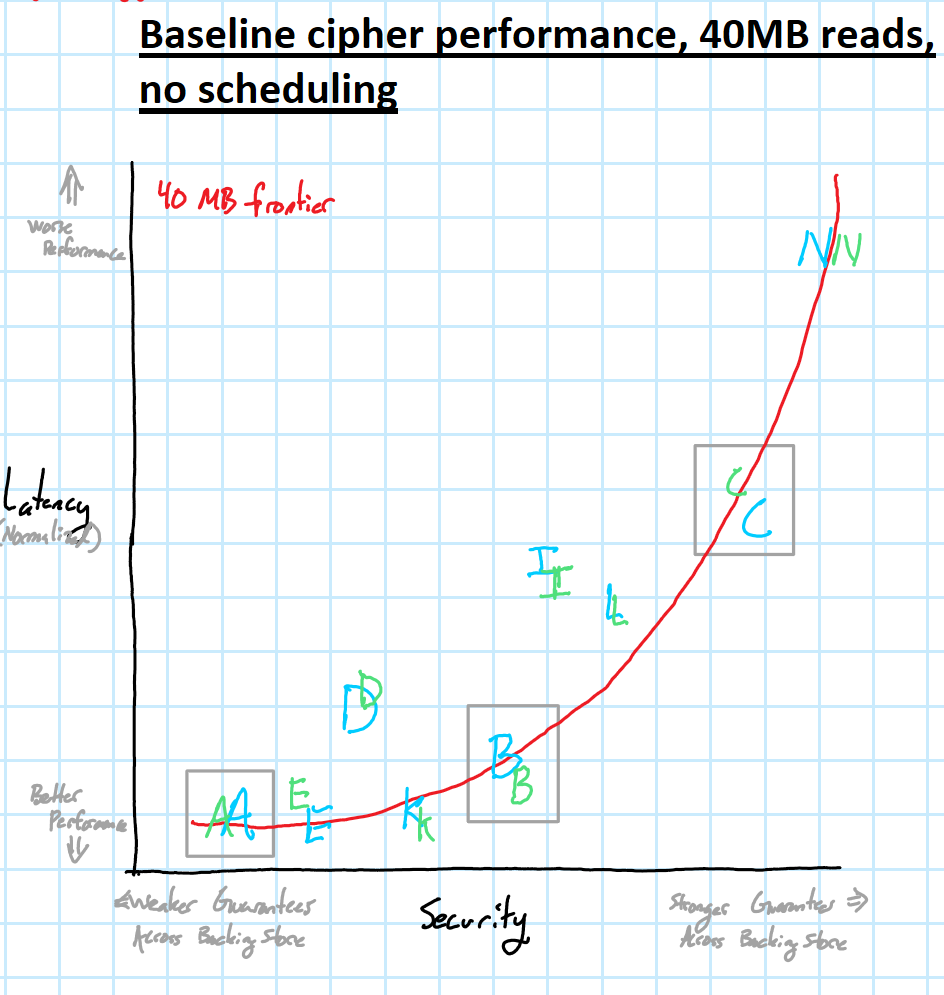
\includegraphics[width=0.8\linewidth]{drawn/1.png}
   \caption{\TODO{Caption goes here}\TODO{No curve in this version!}}\label{fig:40mb-read-frontier}
\end{figure}

\figref{fig:40mb-read-frontier} shows.

\begin{figure}[ht]
 \centering
  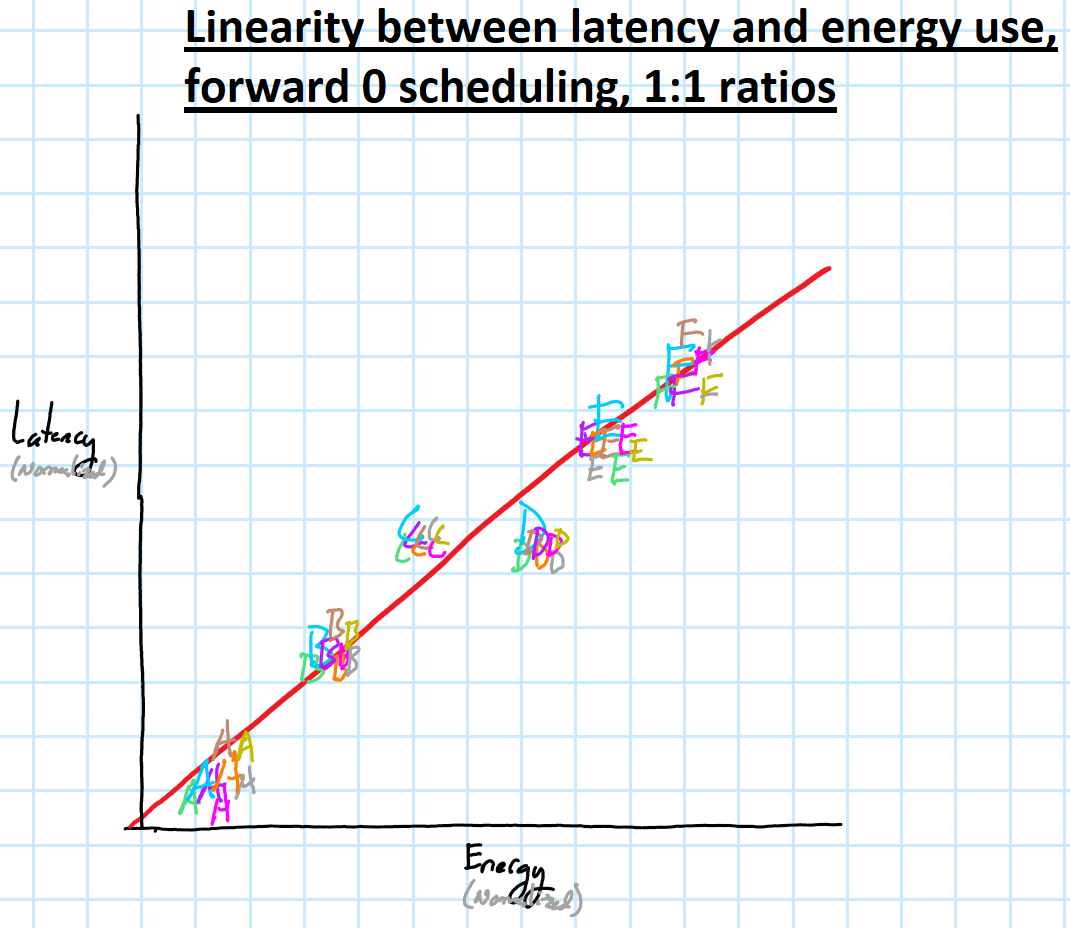
\includegraphics[width=0.8\linewidth]{drawn/5.png}
   \caption{\TODO{Caption goes here}}\label{fig:energy-latency-linearity}
\end{figure}

\subsection{The Need for Dynamic Tradeoff Management}

\subsubsection{Example A's Name Goes Here}

\subsubsection{Example B's Name Goes Here}
